%
% teil3.tex -- Beispiel-File für Teil 3
%
% (c) 2020 Prof Dr Andreas Müller, Hochschule Rapperswil
%
% !TEX root = ../../buch.tex
% !TEX encoding = UTF-8
%
\subsection{Mutation
\label{buch:paper:varalg:subsection:mutation}}
\index{Mutation}%
Dieser Schritt sorgt dafür, dass zufällige Änderungen in den Genen 
stattfinden. Dadurch entstehen neue Variationen, welche in der 
Kreuzung nicht entstanden wären und der gesamte Lösungsraum wird 
vergrössert. Zusätzlich soll dieser Schritt verhindern, dass nach 
einer Anzahl von Generationen immer wieder die gleichen 
Genmuster entstehen und der Algorithmus in einem lokalen Extrempunkt 
stecken bleibt.
Die Mutation tritt nicht bei jedem Nachkommen auf, sondern wird, 
ähnlich wie in der Natur, zufällig ausgelöst. Dazu wird eine Bedingung 
der Form \( \text{Zufällige Zahl} < \text{Grenzzahl} \) definiert. 
Je kleiner die Grenzzahl, desto unwahrscheinlicher ist eine Mutation. 
Die Grenzzahl wird im Voraus festgelegt und liegt im Intervall \([0,1]\).
Nun kann über den String iteriert werden, wobei an jeder Position eine 
zufällige Zahl generiert wird, die ebenfalls im Intervall \([0,1]\) 
liegt. Wird die Bedingung erfüllt, wird die entsprechende Stelle, 
wie in Abbildung \ref{fig:mutation_genetic_string} dargestellt,
invertiert.
\begin{figure}
	\centering
	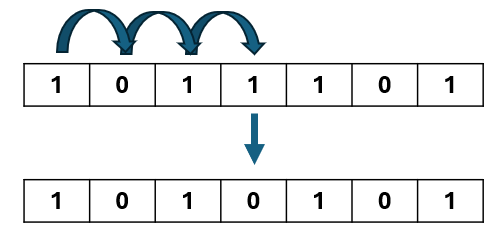
\includegraphics[width=0.8\textwidth]{
        papers/varalg/images/teil3/09GeneticStringMutation.png
        }
	\caption{
	Beispiel einer Mutation mit einem genetischen String aus 0 und 1. Die
	Mutation wird zufällig ausgelöst und invertiert die Stelle.
	}
	\label{fig:mutation_genetic_string}
\end{figure}

\subsubsection{Mutation auf das TSP angepasst
\label{buch:paper:varalg:subsection:mutation_tsp}}
Für das Travelling-Salesman-Problem wird die Mutation so angepasst,
dass, wenn eine Mutation stattfindet, zwei zufällige Stellen ausgewählt
und diese Städte vertauscht werden, 
wie in der Abbildung \ref{fig:mutation_genetic_string_cities}.
\begin{figure}
	\centering
	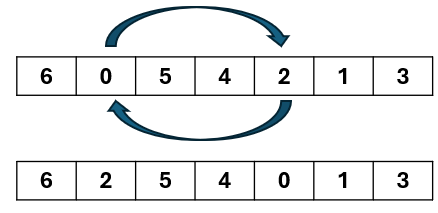
\includegraphics[width=0.8\textwidth]{
        papers/varalg/images/teil3/09GeneticStringCitiesMutation.png
        }
	\caption{Beispiel einer Mutation mit Städten}
	\label{fig:mutation_genetic_string_cities}
\end{figure}
